\begin{figure}[ht]
    \centering
    \begin{subfigure}[t]{0.5\textwidth}
        \centering
        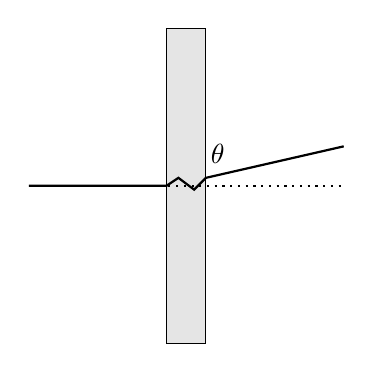
\begin{tikzpicture}
            \draw[fill=gray!20] (-0.25,-2) rectangle (0.25,2);
            \draw[black, thick, dotted] (-2,0) -- (2,0);
            \draw[black, thick] (-2,0) -- (-0.25,0) -- (-0.1,0.1) -- (0.1,-0.05) -- (0.25,0.1) -- (2,0.5);
            \node at (0.4,0.4) {$\theta$};
        \end{tikzpicture}
        \caption{Thin scatterer}
    \end{subfigure}%
    ~
    \begin{subfigure}[t]{0.5\textwidth}
        \centering
        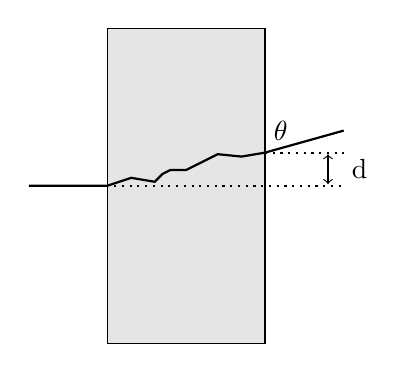
\begin{tikzpicture}
            \draw[fill=gray!20] (-1,-2) rectangle (1,2);
            \draw[black, thick, dotted] (-2,0) -- (2,0);
            \draw[black, thick] (-2,0) -- (-1,0) -- (-0.7,0.1) -- (-0.4,0.05) -- (-0.3,0.15) -- (-0.2,0.2) -- (0,0.2) -- (0.3,0.35) -- (0.4,0.4) -- (0.7,0.37) -- (1,0.42) -- (2,0.7);
            \draw[black, thick, dotted] (1,0.42) -- (2,0.42);
            \draw [<->] (1.8,0.02) -- (1.8,0.40);
            \node at (2.2,0.21) {d};
            \node at (1.2,0.7) {$\theta$};
        \end{tikzpicture}
        \caption{Thick scatterer}
        \label{fig:dev/dense/scatterers/thick}
    \end{subfigure}
    \caption{Illustration of a particle passing through (a) a thin and (b) a thick scatterer. Due to the thickness of the scatterer, the particle will have a positional offset to the unimpeeded trajectory.}
    \label{fig:dev/dense/scatterers}
\end{figure}
